\documentclass[runningheads]{llncs}

% Required packages from ECML-PKDD template
\usepackage[T1]{fontenc}
\usepackage{graphicx}
\usepackage{booktabs}
\usepackage[misc]{ifsym}
\newcommand{\corr}{(\Letter)}

% Additional packages (compatible with llncs)
\usepackage{amsmath}
\usepackage{amssymb}
\usepackage{multirow}
\usepackage{enumitem}
\usepackage{float}
\usepackage{adjustbox}
\usepackage{hyperref}
\usepackage{xcolor}
\usepackage{url}
\usepackage{longtable}
% \usepackage{microtype}  % Removed - incompatible with llncs

% Line spacing - llncs compliant
\setlength{\textfloatsep}{6pt plus 2pt minus 2pt}
\setlength{\dbltextfloatsep}{6pt plus 2pt minus 2pt}

\begin{document}

\title{FIG-MAC: A Fine-grained Inspiration Graph Empowered Multi-Agent Collaboration for Automated Scientific Hypothesis Generation}

\titlerunning{FIG-MAC for ASHG}

\author{First Author \and Second Author \and Third Author}

\authorrunning{F. Author et al.}

\institute{Affiliation/Address line 1 \\
Affiliation/Address line 2 \\
\email{email@domain}}

\maketitle

\begin{abstract}
Automated Scientific Hypothesis Generation (ASHG) leveraging large language models (LLMs) aims to harness their strengths in knowledge integration, logical reasoning, and text generation for efficiently producing innovative, verifiable scientific hypotheses. However, existing approaches face three critical limitations: (i) insufficient fine-grained knowledge representation, as unstructured context impairs LLM comprehension and reasoning; (ii) lack of knowledge evolution traceability, constraining the generation of innovative cross-domain conjectures; (iii) absence of human-inspired and role-specialized multi-agent collaboration, failing to leverage the efficient innovation mechanisms arising from cognitive diversity and division of labor among expert roles to complete the full ASHG-evaluation loop. To address these limitations, we propose the Fine-grained Inspiration Graph-empowered Multi-Agent Collaboration framework (FIG-MAC) including: (i) Fine-grained Inspiration Graph module (FIG), to obtain fine-grained structured knowledge representations, where nodes represent academic semantic units and edges encode heuristic relationships among them; (ii) "Skeleton-Flesh" hybrid reasoning module, fusing FIG-based graph path reasoning as a structural backbone with vector search as semantic enrichment, to obtain the traceable scientific conjecture paths; (iii) role-specialized Multi-Agent framework, inspired by real scientific teamwork, enabling a closed-loop process of scientific conjecture generation, screening, and validation. Experiments results demonstrate that FIG-MAC significantly outperforms state-of-the-art methods on source diversity, provenance-adjusted novelty, and raw novelty.
%Our code is available at \href{https://github.com/SiyuanChenToDo/KG-LLM.git}{GitHub repository}.

%1细粒度的知识表示影响llm准确性，2没有办法捕捉跨领域知识演化轨迹，限制了跨领域创新猜想提出，3没有借鉴不同角色协作的高效创新
\keywords{Scientific Hypothesis Generation, Multi-Agent Collaboration, Knowledge Graphs, Large Language Models}
\end{abstract}

\section{Introduction}

Automated Scientific Hypothesis Generation (ASHG) based on large language models (LLMs) aims to leverage their robust capabilities in knowledge integration, logical reasoning, and text generation to efficiently produce innovative and verifiable scientific hypotheses~\cite{DBLP:journals/tmlr/AgarwalSPLDSCP25,DBLP:journals/pr/LiuZWL26}. As illustrated in Figure~\ref{fig1}, such methods have achieved initial success in multiple domains, including the prediction of chemical molecular properties~\cite{yang2024moose,yang2025moose2}, the formulation of physical theoretical conjectures, the screening of novel semiconductor materials, and the mining of potential drug molecules.

\begin{figure}[t]
    \centering 
    
\includegraphics[width=1\textwidth]{fig1.pdf} 
    \caption{The Wide-Ranging Applications of ASHG Across Diverse Domains.}
    \label{fig1}
\end{figure}

In recent years, ASHG focus on three domains: (1) to identify potential research gaps in academic literature, models such as AutoResearcher~\cite{DBLP:journals/corr/abs-2510-20844}, HypoGen~\cite{zhou2024hypothesis}, and MC-NEST~\cite{DBLP:journals/corr/abs-2411-15645} detect research blind spots by integrating knowledge retrieval and logical reasoning; (2) to improve the empirical feasibility and verifiability of generated hypotheses, AI Scientist systems~\cite{DBLP:journals/corr/abs-2408-06292,aiscientist_v2} operationalize hypothesis generation as an iterative “proposing-evaluating-refining” loop, Causal Graph-guided approaches~\cite{tong2024automating} constrain hypothesis space using explicit causal structures, and LLM-based iterative optimization~\cite{rabby2025iterative} progressively refines hypotheses via feedback-driven reasoning and evaluation; (3) to improve the factual consistency and verifiability of hypotheses, techniques including Retrieval-Augmented Generation (RAG)~\cite{DBLP:conf/nips/LewisPPPKGKLYR020} and Graph Reasoning~\cite{liang2024survey} are used to enhance the scientific rigor and reliability of hypotheses.

However, the following limitations remain: (1) insufficient fine-grained academic knowledge representation: Most existing external knowledge represent only abstract-level information,  leading to coarse-grained representations and lacking complete logical links among scientific knowledge. Such unstructured knowledge  affect the subsequent comprehension and reasoning accuracy of LLMs; 
(2) lack of traceability knowledge evolution: Current knowledge reasoning based on surface-level semantic similarity or citation associations, lacking modeling of the origin and evolution path of knowledge. This makes it difficult for models to understand the dynamic process of ASHG and restricts their ability to transcend the boundaries of existing knowledge domains, constraining the generation of innovative cross-domain conjectures;
(3) absence of structured, role-aware multi-agent collaboration: Single agent cannot independently complete the full-process closed loop from problem discovery and reasoning generation to hypothesis evaluation.
%Insufficient exploration of multi-agent collaboration mechanisms has hindered the large-scale practical deployment of ASHG methods.


%补充语义单元解释
To address these challenges, we propose the Fine-grained Inspiration Graph-empowered Multi-Agent Collaboration framework (FIG-MAC). First, the Fine-grained Inspiration Graph (FIG) module transforms raw corpus into structured semantic units (abstract, core problem, related work, preliminary innovation analysis, 2–4 research questions and corresponding solutions proposed in the paper, and framework summary, among others) through knowledge parsing and constructs relationships between these units, providing structured knowledge for reasoning. Second, the "Skeleton-Flesh" hybrid reasoning module generates knowledge evolution paths (the "Skeleton") via graph traversal, and supplements specific content (the "Flesh") for each node by combining vector retrieval, forming a traceable dynamic knowledge context. Finally, the role-specialized Multi-Agent framework simulates the real scientific research process by setting intelligent roles such as knowledge exploration, idea generation, and parallel domain review. Through multiple rounds of evaluation and knowledge interpretability feedback, the framework generates rigorously verified scientific hypotheses. Extensive experiments demonstrate that FIG-MAC significantly outperforms state-of-the-art methods: improving source diversity by 26.9\%, provenance-adjusted novelty by 55.1\%, and raw overall novelty by 31.8\% compared to the best baseline.

Our contributions are summarized as follows:

\noindent\textbullet\ \textbf{Multi-Agent Collaboration Framework for ASHG.} We design a role-specialized multi-agent system that simulates real scientific teamwork through a closed-loop process where generation, evaluation, and validation are tightly coupled, ensuring hypotheses are both innovative and scientifically rigorous.

\noindent\textbullet\ \textbf{Fine-grained Inspiration Graph (FIG).} We construct a heterogeneous knowledge graph that decomposes papers into fine-grained semantic units and introduces  \textit{Inspired} edges to explicitly model cross-paper innovation pathways. This design enables structured denoising of academic knowledge and captures innovation mechanisms invisible to traditional methods.

\noindent\textbullet\ \textbf{"Skeleton-Flesh" Hybrid Reasoning.} We propose a dual-path reasoning mechanism where graph traversal discovers cross-domain knowledge evolution paths  and vector retrieval enriches them with domain-specific technical details. This hybrid approach ensures generated hypotheses achieve both structural novelty through cross-domain connections and technical feasibility through grounded semantic evidence.


\section{Related Work}
%按照科学猜想流程介绍
\subsection{Semantic Retrieval in Scientific Contexts}
Scientific paper retrieval employs queries like abstracts/titles \cite{singh2023scincl,ostendorff2022neighborhood,cohan2020specter}, keywords \cite{sesagiri2017full}, textual queries \cite{anand2017proposed,parisot2022scientific,medic2023similarity} or paper aspects \cite{singh2024scispace,singh2023scincl,mysore2022multi,ostendorff2022s2orc}, relying on semantic similarity for representation learning. However, mainstream retrieval models (sentence-based similarity \cite{reimers2019sentence,beltagy2019scibert} or generic inter-document embedding \cite{cohan2020specter,singh2022specter2}) often yield irrelevant results (e.g., keyword overlap). Recent studies highlight semantic similarity's ineffectiveness for scientific retrieval \cite{yang2024c}, emphasizing the need for deeper analysis of solution applicability to target problems.

\subsection{From Literature-Based Discovery to LLM-Based Generation}
Automated scientific hypothesis generation has evolved from traditional statistical methods to modern deep learning approaches. Literature-Based Discovery (LBD) is rooted in "undiscovered public knowledge" and the ABC model infers relationships between concepts $A$ and $C$ via shared intermediate concepts $B$ \cite{swanson1986fish,swanson1986undiscovered}. Recent LLM-based approaches enhance hypothesis generation through agentic frameworks \cite{wang2024research,si2024large,baek2025research}, but neglect retrieval quality, limiting hypothesis novelty, validity and diversity \cite{lewis2020retrieval,zhao2024survey,li2024b}. While some methods incorporate knowledge subgraphs, citation neighbors or semantically similar works \cite{wang2024research,li2024b,baek2025research}, seed paper abstracts (containing methodology/results) introduce retrieval bias and reduce idea novelty.


\subsection{Structured Knowledge based Collaborative Validation}
Knowledge graph-based approaches frame hypothesis generation as link prediction over structured scientific knowledge \cite{borrego2025research,de2021discovering}. Early academic knowledge graphs (Semantic Scholar \cite{ammar2018construction}, Microsoft Academic Graph \cite{wang2020microsoft}) model coarse-grained entities (papers, authors, venues) and citations, while recent work focuses on fine-grained entity/relationship modeling \cite{luan2018multi} for precise hypothesis generation. Graph embedding methods score hypothesis plausibility via low-dimensional entity/relation representations \cite{rossi2021knowledge,wang2021survey}.

Multi-agent systems enable collaborative hypothesis generation/validation by distributing roles (generation, critique, refinement) across specialized agents \cite{ghafarollahi2025sciagents,ke2025biodisco}. SciAgents integrates ontological knowledge graphs with LLMs via specialized agents (Ontologist, Scientists, Critic) \cite{ghafarollahi2025sciagents}, and frameworks like POPPER implement agentic validation based on falsification \cite{huang2025automated}.\\


Existing methods suffer from critical limitations: over-reliance on shallow semantic similarity/static graph links (ignoring dynamic knowledge evolution and closed-loop evaluation), lack of unified frameworks for discovery, reasoning traceability and multi-agent evaluation, and separation of hypothesis generation/validation (hindering iterative refinement via empirical feedback). Our work addresses these gaps with an integrated framework combining fine-grained knowledge construction, traceable reasoning paths, and role-specialized multi-agent collaboration for hypothesis generation and validation.


\section{Methodology}
\label{sec:methodology}

We propose FIG-MAC, a collaborative multi-agent framework designed for ASHG by simulating the reasoning process of human research teams. As illustrated in Figure~\ref{fig2}, FIG-MAC consists of three interconnected modules that form a complete hypothesis generation pipeline.

\textbf{Module 1: Fine-grained Inspiration Graph (FIG).} This module serves as the structured knowledge foundation. Raw academic papers first undergo semantic parsing to extract 21 semantic units including research questions (RQs), solutions (SOLs), and metadata. These units form a heterogeneous knowledge graph with three entity types: papers (PAP), research questions (RQ), and solutions (SOL). The graph encodes two critical relation types: hierarchical relations ($r_{\text{has\_rq}}$, $r_{\text{has\_sol}}$) modeling intra-paper structure, and cross-paper relations ($r_{\text{related}}$, $r_{\text{inspired}}$) capturing innovation pathways between papers. An RGCN-based link prediction mechanism discovers latent inspiration paths connecting solutions from one paper to research questions in others, enabling cross-domain knowledge discovery that transcends citation networks.

\textbf{Module 2: ``Skeleton-Flesh'' Hybrid Reasoning.} Given a user query, this module retrieves relevant knowledge through complementary pathways. The ``Skeleton'' path performs graph traversal on FIG to identify inspiration chains---multi-hop paths connecting the query to relevant solutions through intermediate research questions. These chains provide structural novelty by linking seemingly unrelated domains. Simultaneously, the ``Flesh'' path conducts vector-based dense retrieval to gather domain-specific technical details from recent papers. A composite scoring function (Eq.~\ref{eq:score}) ranks candidate paths by combining query relevance, structural confidence, and target coherence. The merged ``Skeleton-Flesh'' output forms a traceable, semantically enriched knowledge context that grounds hypothesis generation in both cross-domain structural insights and contemporary technical feasibility.

\textbf{Module 3: Role-Specialized Multi-Agent Framework.} Eight specialized agents collaborate through a state-driven workflow to generate and refine hypotheses. The process begins with \textit{Scholar Scour} (Research Assistant) conducting literature review using the hybrid retrieval results. \textit{Idea Igniter} (Innovator) then generates candidate hypotheses by synthesizing cross-domain insights from the inspiration chains. Three parallel reviewers---\textit{Dr. Qwen Technical} (Technical Reviewer), \textit{Dr. Qwen Practical} (Practical Reviewer), and \textit{Prof. Qwen Ethics} (Ethical Reviewer)---independently assess the proposal across five dimensions (novelty, significance, effectiveness, clarity, feasibility) via confidence-aware weighted aggregation. \textit{Dr. Qwen Leader} (Coordinator) synthesizes the reviews into a structured report. If quality thresholds are unmet, \textit{Critic Crucible} (Quality Controller) provides detailed feedback triggering revision cycles. Finally, \textit{Prof. Qwen Editor} polishes the output into a publication-ready hypothesis. This closed-loop process iterates up to 3 times, with dual-memory context management preserving critical feedback across iterations while mitigating confirmation bias.

% \textbf{Notation.} Throughout this section, we use the following notation: $\mathcal{G} = (\mathcal{V}, \mathcal{E}, \mathcal{R})$ denotes a heterogeneous knowledge graph with node set $\mathcal{V}$, edge set $\mathcal{E}$, and relation type set $\mathcal{R}$; $\mathcal{C}$ denotes the shared context space containing retrieval evidence and inter-agent messages; bold uppercase letters (e.g., $\mathbf{W}$, $\mathbf{h}$) represent matrices and vectors; calligraphic letters (e.g., $\mathcal{S}$, $\mathcal{A}$) denote sets and spaces; subscripts indicate entity indices (e.g., $i$, $j$) or relation types (e.g., $r$); superscripts in parentheses (e.g., $^{(l)}$, $^{(t)}$) indicate layer numbers or time steps.

\begin{figure*}[t] 
\centering
    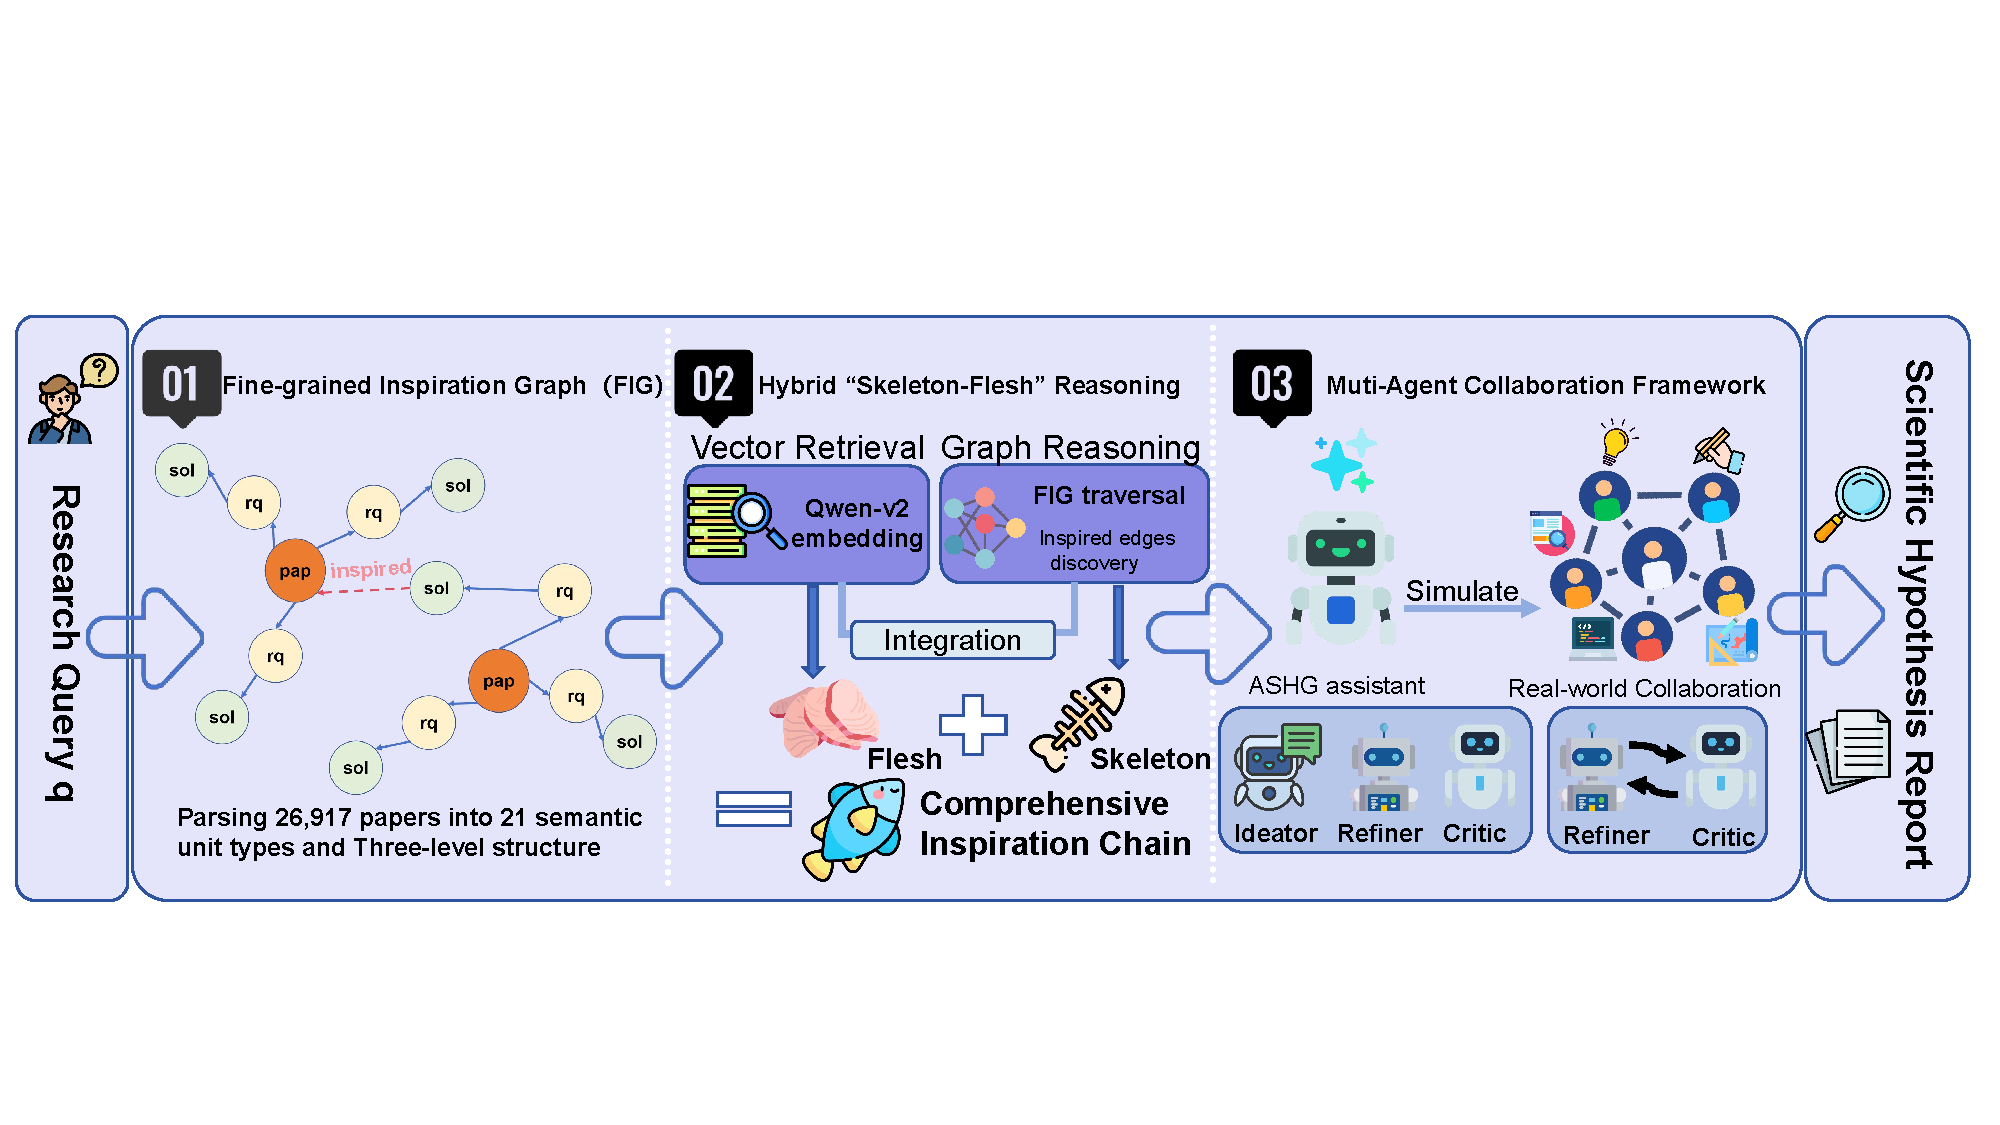
\includegraphics[width=1\textwidth]{fig2.pdf} 
    \caption{The FIG-MAC framework architecture comprising three integrated modules: (\textbf{a}) The \textit{Fine-grained Inspiration Graph (FIG)} module constructs a heterogeneous knowledge graph from academic papers, with papers (PAP), research questions (RQ), and solutions (SOL) as nodes, and hierarchical relations ($r_{\text{has\_rq}}$, $r_{\text{has\_sol}}$) and cross-paper inspiration relations ($r_{\text{inspired}}$) as edges; (\textbf{b}) The \textit{``Skeleton-Flesh'' Hybrid Reasoning} module combines graph-based path discovery (``Skeleton'') to identify cross-domain inspiration chains connecting queries to solutions via intermediate RQs, with vector-based semantic retrieval (``Flesh'') to enrich paths with domain-specific technical details from recent papers; (\textbf{c}) The \textit{Role-Specialized Multi-Agent} module orchestrates eight specialized agents through a state-driven workflow: Scholar Scour conducts literature review, Idea Igniter generates hypotheses, three parallel reviewers (Technical, Practical, Ethical) assess quality dimensions, Dr. Qwen Leader synthesizes reports, Critic Crucible provides revision feedback, and Prof. Qwen Editor produces the final polished hypothesis. The framework iterates until quality thresholds are met, with dual-memory context management preserving critical feedback across revision cycles.}
    \label{fig2}
\end{figure*}

\subsection{Fine-grained Inspiration Graph Construction}
\label{sec:graph_construction}

To enable structured knowledge representation that captures fine-grained academic semantics and cross-paper innovation pathways, we design the Fine-grained Inspiration Graph (FIG). FIG decomposes scientific literature into semantic units and models their relationships at multiple granularities. Formally, FIG is a heterogeneous knowledge graph denoted as $\mathcal{G} = (\mathcal{V}, \mathcal{E}, \mathcal{R})$, where $\mathcal{V}$ represents the set of nodes, $\mathcal{E}$ denotes the set of edges, and $\mathcal{R}$ is the set of relation types. The current implementation yields three primary entity types: $PAP$ (Papers), $RQ$ (Research Questions), and $SOL$ (Solutions).

\textbf{Fine-grained Data Structuring.} The core challenge lies in accurately extracting key information and core entities from raw text. We perform fine-grained structured parsing on each paper, dividing the full text into 21 semantic units \textit{instances} across 8 core \textit{types} (Table~\ref{tab:semantic_prompt_extraction}). These instances are categorized into three groups:
\begin{itemize}[leftmargin=*]
    \item \textbf{Metadata Attributes (8 instances):} DOI, title, authors, year, conference, venue, citation count, and abstract, providing bibliographic context for each paper.
    \item \textbf{Core Content Attributes (9 instances):} Core problem, related work, preliminary innovation analysis, up to 4 research questions (RQ 1--4) with their simplified versions, up to 4 solutions (SOL 1--4) with their simplified versions, and framework summary. These form the primary knowledge units for the PAP-RQ-SOL hierarchy.
    \item \textbf{Auxiliary Attributes (4 instances):} Additional semantic annotations supporting entity disambiguation and relationship inference.
\end{itemize}
This categorization ultimately forms a three-level knowledge structure centered on the core entities "PAP - RQ - SOL", with metadata and auxiliary attributes serving as supplementary information for retrieval and reasoning.

\textbf{Entity Extraction.} Papers are manually annotated and refined to standardized samples. And we fine-tune a Qwen-based llm as a extractor. This model then processes the full corpus, generating structured semantic units for each paper.

\textbf{Relation Construction.} FIG encodes two relation classes: (1) Hierarchical relations $r_{\text{has\_rq}}$ (connects a paper $PAP_i$ to its research question $RQ_j$) and $r_{\text{has\_sol}}$ (connects a research question $RQ_i$ to its solution $SOL_j$) mapping intra-paper structures where each paper contains approximately 3 research questions on average (based on experiments); and (2) Cross-paper relations $r_{\text{related}}$ (connects semantically similar entities across different papers) and $r_{\text{inspired}}$ (connects a solution $SOL_i$ from one paper to a research question $RQ_j$ or methodology in another paper, capturing cross-paper innovation pathways) capturing inter-paper influences.

To construct cross-paper edges at scale, we combine similarity filtering with supervised classification. Samples are manually labeled by three experts into three categories: Related, Inspired, or Irrelevant. Pairs with similarity below threshold are pruned. Remaining candidates are classified by a fine-tuned Qwen3-8B. Critically, $r_{\text{inspired}}$ edges explicitly model how $SOL$ in one paper inspire $RQ$ or methodologies in another, capturing innovation pathways invisible to citation analysis.

To discover invisible inspiration paths, we employ a Relation Graph Convolutional Network (RGCN) for representation learning. Let $\mathbf{h}_i^{(l)} \in \mathbb{R}^d$ denote the embedding of node $i$ at layer $l$, where $d$ is the embedding dimension. The RGCN update rule is:
\begin{equation}
    \mathbf{h}_i^{(l+1)} = \sigma \Bigg( \sum_{r \in \mathcal{R}} \sum_{j \in \mathcal{N}_r(i)} \frac{1}{|\mathcal{N}_r(i)|} \mathbf{W}_r^{(l)} \mathbf{h}_j^{(l)} + \mathbf{W}_0^{(l)} \mathbf{h}_i^{(l)} \Bigg),
\end{equation}
where $\mathcal{N}_r(i) = \{j \mid (j, i, r) \in \mathcal{E}\}$ denotes the set of neighbors of node $i$ under relation $r \in \mathcal{R}$; $\mathbf{W}_r^{(l)} \in \mathbb{R}^{d \times d}$ is the relation-specific weight matrix at layer $l$; $\mathbf{W}_0^{(l)} \in \mathbb{R}^{d \times d}$ is the self-connection weight matrix; and $\sigma(\cdot)$ is the activation function (ReLU).

After $L$ layers, we obtain final node embeddings $\mathbf{h}_i^L$. These are decoded via the DistMult scoring function $s$ to predict missing links:
\begin{equation}
    s(u, r, v) = (\mathbf{h}_u^L)^T \mathbf{R}_r \mathbf{h}_v^L,
\end{equation}
where $(u, r, v)$ denotes a triple consisting of head entity $u \in \mathcal{V}$, relation $r \in \mathcal{R}$, and tail entity $v \in \mathcal{V}$; $\mathbf{R}_r \in \mathbb{R}^{d \times d}$ is a learnable diagonal matrix representing relation $r$.

% \textbf{From Local Triple Scoring to Global Chain Discovery.} DistMult evaluates the plausibility of \textit{individual} triples but cannot assess the coherence of multi-hop paths. To construct inspiration chains, we employ a two-stage process:

% \textit{Step 1: Local Triple Filtering.} DistMult assigns a confidence score $s(u, r, v)$ to each candidate triple, filtering out low-confidence links. Only triples with scores above a threshold are retained as ``valid components'' for path construction.

% \textit{Step 2: Beam Search for Chain Construction.} Starting from the entry node $\text{RQ}_0$ (most similar to the query), beam search iteratively expands paths using only the high-confidence triples from Step 1. At each hop, it maintains the top-$k$ most promising partial paths (where $k$ is the beam width), pruning inferior candidates to control computational complexity. This yields a set of complete inspiration chains $\pi = \{(v_1, r_1, v_2), (v_2, r_2, v_3), \ldots, (v_m, r_m, v_{m+1})\}$ connecting source solutions to target research questions.

% \textit{Step 3: Global Chain Ranking.} The candidate chains from Step 2 are ranked using the composite scoring function (Eq.~\ref{eq:score}), which combines query relevance, structural confidence (DistMult scores), and target coherence to select the final inspiration chains.

\subsection{"Skeleton-Flesh" Hybrid Reasoning Module}
\label{sec:hybrid_reasoning}

To achieve deep, traceable reasoning that combines the semantic richness of dense retrieval with the structural insights of graph traversal, we propose a Hybrid ``Skeleton-Flesh'' Reasoning method. This approach integrates two complementary retrieval paradigms: graph-based path discovery provides the ``skeleton'' of cross-domain knowledge evolution, while vector-based semantic search provides the ``flesh'' of domain-specific technical details. Given a research query $Q$, two retrieval functions operate in parallel: (1) VectorEnrichment $\mathcal{R}_V(Q)$ identifies topically relevant papers via dense embeddings, returning papers ranked by semantic similarity; (2) \text{GraphSkeleton} $\mathcal{R}_G(Q)$ traverses FIG to extract inspiration chains $\pi$ connecting $Q$ to $\text{SOL}$ nodes through $r_{\text{inspired}}$ edges.

The integration function $\mathcal{I}$ merges structural backbones with semantic evidence:
\begin{equation}
    \mathcal{I}(\mathcal{R}_V, \mathcal{R}_G) = \text{GraphSkeleton}(\mathcal{R}_G) \cup \text{VectorEnrichment}(\mathcal{R}_V),
\end{equation}
where $\text{GraphSkeleton}(\mathcal{R}_G)$ extracts cross-domain knowledge evolution paths from FIG, and $\text{VectorEnrichment}(\mathcal{R}_V)$ supplements domain-specific technical details. The resulting $\mathcal{I}$ forms a semantically enriched evolutionary subgraph that traces how knowledge progresses across domains while maintaining technical grounding.

Each inspiration chain $\pi = (\text{RQ}_0, \text{RQ}_1, \ldots, \text{RQ}_m, \text{SOL}_j, \text{PAP}_k)$ is ranked by a composite scoring function:
\begin{equation}
    \text{score}(\pi) = \alpha \cdot \text{sim}(Q, \text{RQ}_0) + \beta \cdot \text{conf}(\text{RQ}_m \rightarrow \text{SOL}_j) + \gamma \cdot \text{conf}(\text{SOL}_j \rightarrow \text{PAP}_k),
    \label{eq:score}
\end{equation}
where $Q$ denotes the input research question; $\text{RQ}_0$ is the entry research question node in FIG most similar to $Q$; $\text{RQ}_1, \ldots, \text{RQ}_m$ are intermediate research question nodes forming the evolution path; $\text{SOL}_j$ is the solution node; and $\text{PAP}_k$ is the target paper node. The term $\text{sim}(Q, \text{RQ}_0) \in [0, 1]$ measures cosine similarity between query and path start node. The confidence $\text{conf}(\text{RQ}_m \rightarrow \text{SOL}_j) = s(\text{RQ}_m, r, \text{SOL}_j)$ is the RGCN-predicted score for edge $r \in \{r_{\text{has\_sol}}, r_{\text{inspired}}\}$ connecting the final research question to solution, where $r_{\text{has\_sol}}$ denotes the hierarchical has-solution relation and $r_{\text{inspired}}$ denotes the cross-paper inspiration relation. The confidence $\text{conf}(\text{SOL}_j \rightarrow \text{PAP}_k) = s(\text{SOL}_j, r_{\text{inspired}}, \text{PAP}_k)$ is the score for the inspired edge from solution to target paper. Finally, $\alpha, \beta, \gamma \in [0, 1]$ are hyperparameters satisfying $\alpha + \beta + \gamma = 1$ that balance query relevance, structural confidence, and target coherence. Multiple high-scoring paths are extracted via beam search to form the complete set of inspiration chains. This dual-path mechanism ensures that generated hypotheses achieve both structural novelty (through cross-domain graph paths that connect seemingly unrelated research areas) and technical feasibility (through vector-grounded domain-specific details), addressing the fundamental challenge of generating ideas that are innovative yet empirically realizable.

\subsection{Role-Specialized Multi-Agent Framework}
\label{sec:workflow}

To enable collaborative hypothesis generation that mimics the coordination and brainstorming dynamics of real research teams, we design a Multi-Agent Collaboration framework with multiple specialized agent roles. Rather than employing a single monolithic model, this framework assigns distinct responsibilities to different agent types---including research assistants for evidence gathering, innovators for hypothesis drafting, domain reviewers for parallel assessment, coordinators for synthesis, and quality controllers for refinement. Each agent of type $A_i$ is formalized as a tuple:
\begin{equation}
    A_i = (\mathcal{S}_i, \mathcal{A}_i, \mathcal{O}_i, \sigma_i, \mathcal{M}_i, \mathcal{T}_i),
\end{equation}
where $\mathcal{S}_i$ denotes the state space containing all possible states of agent $i$; $\mathcal{A}_i$ is the action space of available actions; $\mathcal{O}_i: \mathcal{S}_i \rightarrow \mathcal{O}$ is the observation function mapping states to observations; $\sigma_i: \mathcal{S}_i \times \mathcal{C} \rightarrow \Delta(\mathcal{A}_i)$ is the role-specific policy mapping states and context to action probabilities; $\mathcal{M}_i = (M_i^p, M_i^c)$ is the dual-memory structure with persistent memory $M_i^p$ (long-term knowledge) and conversational memory $M_i^c$ (short-term dialogue history); and $\mathcal{T}_i$ is the tool set providing external capabilities.

State evolution follows a Markov decision process. At time step $t$, agent $i$ observes $o_i^{(t)} = \mathcal{O}_i(s_i^{(t)})$, takes action $a_i^{(t)}$ sampled from policy $\sigma_i$, and transitions to next state $s_i^{(t+1)}$:
\begin{align}
    s_i^{(t+1)} &= f_i\big(s_i^{(t)}, a_i^{(t)}, o_i^{(t)}, \mathcal{C}^{(t)}\big), \\
    a_i^{(t)} &\sim \sigma_i\big(s_i^{(t)}, \mathcal{C}^{(t)}\big),
\end{align}
where $f_i$ is the state transition function and $\mathcal{C}^{(t)}$ is the shared context aggregated from retrieval evidence and inter-agent messages at time $t$.

\textbf{Agent Roles.} The framework comprises seven functional role types, each representing a distinct capability required for scientific hypothesis generation: (1)~\textit{Research Assistants} for literature gathering and synthesis; (2)~\textit{Innovators} for hypothesis drafting; (3)~\textit{Technical Reviewers} for scientific validity assessment; (4)~\textit{Practical Reviewers} for feasibility evaluation; (5)~\textit{Ethical Reviewers} for societal impact analysis; (6)~\textit{Coordinators} for perspective integration; and (7)~\textit{Quality Controllers} (including critics, revisers, and editors) for iterative refinement. Each role type can be instantiated by one or more agents depending on workload and parallelism requirements; the seven types represent a complete functional coverage of the research workflow rather than a fixed agent count.

\textbf{Context Management.} To handle context-length constraints, agents prune conversational history by relevance. Let $\mathbf{m}$ denote a message in memory, $s_i$ the current state, and $\Delta t$ the time elapsed since message creation. Each agent selects a pruned memory set $M_i^{c'}$ of maximum size $L_{\max} \in \mathbb{N}^+$:
\begin{equation}
    M_i^{c'} = \arg\max_{\mathcal{M}' \subseteq M_i^c} \sum_{\mathbf{m} \in \mathcal{M}'} \phi(\mathbf{m}, s_i) \quad \text{s.t.} \quad |\mathcal{M}'| \leq L_{\max},
\end{equation}
where $\phi(\mathbf{m}, s_i)$ is the message relevance score balancing recency, semantic similarity, and LLM-judged quality:
\begin{equation}
    \phi(\mathbf{m}, s_i) = \alpha_1 \exp(-\lambda \Delta t) + \beta_1 \cos\big(\text{embed}(\mathbf{m}), \text{embed}(s_i)\big) + \gamma_1 \cdot \text{LLM}_{\text{judge}}(\mathbf{m}),
\end{equation}
where $\exp(-\lambda \Delta t)$ implements exponential decay with rate $\lambda > 0$; $\cos(\cdot, \cdot)$ denotes cosine similarity between message and state embeddings; $\text{LLM}_{\text{judge}}(\mathbf{m}) \in [0, 1]$ is the LLM-assigned importance score; and $\alpha_1, \beta_1, \gamma_1 \in [0, 1]$ are weighting coefficients satisfying $\alpha_1 + \beta_1 + \gamma_1 = 1$. This preserves critical feedback while mitigating confirmation bias.

\textbf{Parallel Review.} During the ANALYSIS phase, three independent reviewers (Technical Reviewer, Practical Reviewer, Ethical Reviewer) operate concurrently. Let $R_k \in \mathbb{R}^5$ denote the review vector from domain~$k$, where $\mathcal{K} = \{\text{Technical}, \text{Practical}, \text{Ethical}\}$, containing scores across five dimensions (Novelty, Significance, Effectiveness, Clarity, Feasibility) aligned with the subjective quality assessment criteria in Section~\ref{sec:main_results}. Reviews are aggregated via confidence-aware weighting:
\begin{align}
    R_{\text{Analysis}} &= \sum_{k \in \mathcal{K}} w_k \cdot \text{normalize}(R_k), \\
    w_k &= \frac{\exp(c(R_k) / \tau)}{\sum_{j \in \mathcal{K}} \exp(c(R_j) / \tau)},
\end{align}
where $w_k \in [0, 1]$ is the normalized confidence weight for reviewer $k$, computed via softmax over the confidence scores; $c(R_k) \in [0, 1]$ is the confidence score of reviewer $k$; $\text{normalize}(\cdot)$ maps raw scores to $[0, 1]$; and $\tau \in \mathbb{R}^+$ is the temperature parameter controlling weight sharpness (lower $\tau$ increases weight disparity). This weighted aggregation ensures high-confidence reviews dominate while preserving diverse perspectives.

\textbf{State-Driven Workflow.} The collaboration follows a finite state machine $\mathcal{SM} = (\mathcal{S}, \mathcal{T}, s_0, s_F)$ comprising: state set $\mathcal{S}$ with seven phases (LITERATURE review to POLISH); transition function $\mathcal{T}: \mathcal{S} \times \mathcal{C} \rightarrow \mathcal{S}$; initial state $s_0 = $ (LITERATURE review); and terminal states $s_F \in \{\text{POLISH}, \text{REVISION}\}$.

After the REVIEW state, the transition is determined by quality assessment:
\begin{equation}
    \mathcal{T}(s_{\text{REVIEW}}, c) =
    \begin{cases}
        \text{POLISH} & \text{if } q_{\text{overall}} \geq \theta \lor i \geq I_{\max}, \\
        \text{REVISION} & \text{otherwise},
    \end{cases}
\end{equation}
where $q_{\text{overall}} \in [0, 10]$ is the overall review score; $\theta \in [0, 10]$ is the quality threshold for acceptance; $i \in \mathbb{N}$ is the current iteration count; and $I_{\max} \in \mathbb{N}^+$ is the maximum iteration budget.

If revision is required, agents with Quality Controller roles (revisers) update the hypothesis based on review feedback:
\begin{align}
    Q_{\text{review}}^{(i)} &= \text{Review}(H^{(i)}), \\
    H^{(i+1)} &= \text{Revise}\big(H^{(i)}, Q_{\text{review}}^{(i)}\big),
\end{align}
where $\text{Review}(\cdot)$ denotes the peer review operation that evaluates the current hypothesis and generates structured feedback (quality scores and improvement suggestions); $\text{Revise}(\cdot, \cdot)$ denotes the revision operation that updates the hypothesis by incorporating the feedback to produce an improved version; $H^{(i)}$ denotes the hypothesis at iteration $i$; and $Q_{\text{review}}^{(i)}$ is the structured feedback from all reviewers. This closed loop mirrors peer review practice, yielding progressively refined hypotheses with traceable justifications.



\section{Experiments}
\subsection{Evaluation Setup}

\textbf{Datasets.} We evaluate FIG-MAC on the Fine-grained Paper Dataset (FPD), which we constructed from five premier conferences (ACL, EMNLP, NAACL, EACL, AAAI) covering natural language processing and artificial intelligence research from 2019 to 2024. The dataset comprises 26,917 high-quality papers with fine-grained semantic annotations, as shown in Table~\ref{tab:dataset_sources}. Each paper is parsed into 21 semantic units forming a three-level knowledge structure centered on "PAP - RQ - SOL". For evaluation, we randomly selected 150 diverse RQs spanning multiple subfields to assess cross-domain ASHG capabilities. To ensure methodological rigor, we partition these into a validation set (50 RQs) for hyperparameter tuning and a test set (100 RQs) for final evaluation. All reported results in Table~\ref{tab:main_results} (main comparison) and Table~\ref{tab:ablation_results} (ablation study) are obtained on the same held-out test set (100 RQs) using optimal hyperparameters determined from the validation set.

\begin{table}[t]
\centering
\small
\caption{Dataset Paper Sources by Conference.}
\label{tab:dataset_sources}
\begin{tabular}{lcccccc}
\toprule
\textbf{Conference} & ACL & EMNLP & NAACL & EACL & AAAI & \textbf{Total} \\
\midrule
\textbf{Paper Counts} & 5,877 & 7,539 & 2,086 & 991 & 10,424 & 26,917 \\
\bottomrule
\end{tabular}
\end{table}

\textbf{Baseline.} We compare our framework with three state-of-the-art methods: (1) Virtual-Scientists (VirSci)~\cite{DBLP:journals/corr/abs-2410-09403}, a multi-agent method with team-based discussion mechanisms; (2) AI Scientist-v2~\cite{DBLP:journals/corr/abs-2408-06292}, an end-to-end agentic method using tree search for discovery; (3) CoI-Agent~\cite{li2024chain}, a framework simulating a chain of ideas for research development.

\textbf{Evaluation Metrics.} To holistically assess the quality of generated hypotheses, we propose a comprehensive \textbf{Multi-Dimensional Evaluation Framework} integrating objective semantic novelty, provenance integrity, and subjective expert assessment. All metrics are computed per hypothesis $h$ with embedding $\mathbf{e}_h \in \mathbb{R}^d$, following the established methodology~\cite{su2025many}.

\textbf{(1) Objective Semantic Novelty.} We quantify innovation via embedding similarity~\cite{shao2020bertpli,shi2023surprising}. For each hypothesis $h$, we retrieve the top-$K=10$ most similar papers from a corpus of $N=26{,}917$ papers and partition them based on publication year: \textit{historical papers} $\mathcal{P}_{\text{past}}$ (published before 2022) and \textit{contemporary papers} $\mathcal{P}_{\text{contemp}}$ (published in 2022 or later). We define three component metrics:

\begin{itemize}[leftmargin=*, itemsep=2pt]
    \item \textbf{Historical Dissimilarity} ($\text{HD} \in [0, 1]$): Measures semantic distance from prior work~\cite{shao2020bertpli},
    \begin{equation}
        \text{HD}(h) = \frac{1}{K} \sum_{p \in \mathcal{P}_{\text{past}}^{(K)}} \big(1 - \cos(\mathbf{e}_h, \mathbf{e}_p)\big),
        \label{eq:hd}
    \end{equation}
    where $\mathbf{e}_p$ denotes the embedding of paper $p$; $\mathcal{P}_{\text{past}}^{(K)}$ denotes the $K$ most dissimilar historical papers (higher dissimilarity indicates greater novelty versus history); and $\cos(\mathbf{a}, \mathbf{b}) = \frac{\mathbf{a} \cdot \mathbf{b}}{\|\mathbf{a}\| \|\mathbf{b}\|}$ is the cosine similarity between two embeddings.
    
    \item \textbf{Contemporary Dissimilarity} ($\text{CD} \in [0, 1]$): Measures distance from recent work to assess feasibility~\cite{wu2019large,fortunato2018science},
    \begin{equation}
        \text{CD}(h) = \frac{1}{K} \sum_{p \in \mathcal{P}_{\text{contemp}}^{(K)}} \big(1 - \cos(\mathbf{e}_h, \mathbf{e}_p)\big),
        \label{eq:cd}
    \end{equation}
    where $\mathcal{P}_{\text{contemp}}^{(K)}$ denotes the $K$ most similar contemporary papers; and lower CD indicates better alignment with current research trends (higher feasibility).
    
    \item \textbf{Contemporary Impact} ($\text{CI} \in [0, 1]$): Citation percentile rank within publication year, computed as~\cite{yang2022gender,alshebli2018preeminence}
    \begin{equation}
        \text{CI}(h) = \frac{1}{K} \sum_{p \in \mathcal{P}_{\text{contemp}}^{(K)}} \text{PercentileRank}(\text{citations}_p \mid \text{year}_p),
        \label{eq:ci}
    \end{equation}
    where $\text{citations}_p$ is the citation count of paper $p$; $\text{year}_p$ is its publication year; $\text{PercentileRank}(c \mid y)$ computes the percentile rank of citation count $c$ among all papers published in year $y$; and higher CI indicates the hypothesis addresses high-impact topics.
\end{itemize}

The \textbf{Raw Overall Novelty} ($\text{ON}_{\text{raw}} \in \mathbb{R}^+$) combines these components:
\begin{equation}
   \text{ON}_{\text{raw}}(h) = \frac{\text{HD}(h) \times \text{CI}(h)}{\text{CD}(h) + \delta},
   \label{eq:on_raw}
\end{equation}
where $\delta = 0.1$ is a smoothing constant preventing division by zero.

For cross-method comparison, we apply \textbf{rank-based normalization} across all $N_{\text{total}}$ hypotheses to obtain Normalized Overall Novelty:
\begin{equation}
    \text{ON}_{\text{norm}}(h) = \frac{\text{rank}\big(\text{ON}_{\text{raw}}(h)\big)}{N_{\text{total}}} \in \left[\frac{1}{N_{\text{total}}}, 1\right],
    \label{eq:on_norm}
\end{equation}
where $N_{\text{total}} = 600$ is the total number of hypotheses evaluated (150 RQs $\times$ 4 methods); $\text{rank}(\cdot)$ assigns ranks from 1 (lowest) to $N_{\text{total}}$ (highest) based on ON$_{\text{raw}}$ values across all hypotheses.

\textbf{(2) Provenance-Adjusted Novelty.} To distinguish genuine innovation from content replication, we incorporate source usage patterns~\cite{lewis2020retrieval}. For RAG-based methods, let $\mathcal{S} = \{s_1, \ldots, s_M\}$ denote the retrieved source documents. We define:

\begin{itemize}[leftmargin=*, itemsep=2pt]
    \item \textbf{Source Similarity} ($S_{\text{src}} \in [0, 1]$): Average similarity between hypothesis and sources,
    \begin{equation}
        S_{\text{src}}(h) = \frac{1}{M} \sum_{i=1}^{M} \cos(\mathbf{e}_h, \mathbf{e}_{s_i}),
        \label{eq:s_src}
    \end{equation}
    where $\mathbf{e}_{s_i}$ denotes the embedding of source document $s_i \in \mathcal{S}$; $M = |\mathcal{S}|$ is the number of retrieved sources; and lower $S_{\text{src}}$ indicates less replication (more divergence from sources).
    
    \item \textbf{Source Diversity} ($U_{\text{src}} \in [0, 1]$): Cross-domain diversity of sources computed as~\cite{zeng2021fresh,shi2023surprising}
    \begin{equation}
        U_{\text{src}}(h) = 1 - \frac{2}{M(M-1)} \sum_{i<j} \cos(\mathbf{e}_{s_i}, \mathbf{e}_{s_j}),
        \label{eq:u_src}
    \end{equation}
    where the sum iterates over all pairs of distinct source documents; $\cos(\mathbf{e}_{s_i}, \mathbf{e}_{s_j})$ measures similarity between sources $s_i$ and $s_j$; and higher $U_{\text{src}}$ indicates sources span diverse domains (better cross-domain synthesis).
\end{itemize}

The \textbf{Provenance Factor} $G \in [0, 1]$ balances replication penalty against diversity reward:
\begin{equation}
    G(h) = \alpha_2 \cdot \big(1 - S_{\text{src}}(h)\big) + \beta_2 \cdot U_{\text{src}}(h),
    \label{eq:provenance_factor}
\end{equation}
where $\alpha_2 = 0.5$ and $\beta_2 = 0.5$ are weighting coefficients for provenance evaluation (distinct from the path-scoring hyperparameters in Eq.~\ref{eq:score}).

The \textbf{Provenance-Adjusted Novelty} $P \in \mathbb{R}^+$ adjusts raw novelty by provenance quality:
\begin{equation}
   P(h) = \text{ON}_{\text{raw}}(h) \times \big[\gamma_2 \cdot G(h) + (1 - \gamma_2)\big],
   \label{eq:p_score}
\end{equation}
where $\gamma_2 = 0.7$ controls the provenance influence (distinct from the path-scoring hyperparameter in Eq.~\ref{eq:score}).

\textbf{(3) Subjective Quality Assessment.} We employ Qwen-Max as an expert reviewer to evaluate hypotheses on five critical dimensions (1--10 scale each)~\cite{gu2024llm,siyang2024novel}: \textbf{Novelty} (originality of the core idea), \textbf{Significance} (importance of the addressed problem), \textbf{Effectiveness} (methodological soundness), \textbf{Clarity} (communication quality), and \textbf{Feasibility} (implementation practicality). This multi-layered approach ensures that generated ideas are not only semantically novel but also technically grounded and scientifically rigorous.

\textbf{Experimental Configuration.} We use a FAISS vector database containing 26,917 computer science papers (2019 to 2024) and a knowledge graph comprising 26,917 PAP, 76,933 RQ, and 76,933 SOL. All methods use Qwen text-embedding-v2 with embedding dimension $d=1536$ for semantic similarity computation.

For RGCN training on FIG, we employ a 2-layer architecture with hidden dimension 256, DistMult decoder, and additive edge feature aggregation. Training uses mini-batch sampling with fanout [25, 20], batch size 512, learning rate 0.0005, dropout 0.1. The graph is split into 80\% training, 10\% validation, and 10\% test sets. We train for 30 epochs with early stopping (evaluated every 200 iterations), achieving validation MRR of 0.4563 and test MRR of 0.4599 on Inspired edge prediction. All experiments are conducted on NVIDIA RTX 5090 GPUs (32GB memory, Driver Version: 580.105.08, CUDA 13.0), using PyTorch 2.0 with DGL 1.1 for graph operations.

\textbf{Statistical Methodology.} We adopt a \textit{paired design} where each of the 150 RQs is evaluated by all methods (FIG-MAC and baselines) under identical conditions, ensuring fair comparison. To ensure reproducibility, we use fixed random seeds (seed=42) and deterministic decoding (temperature=0.0). Due to computational costs (approximately \$0.50 per RQ per method, totaling \$225 for 3 methods), each RQ is evaluated once per method, and we report mean scores across the 150 RQs. 

\textbf{Statistical Testing.} To assess whether FIG-MAC significantly outperforms baselines, we employ \textit{paired statistical tests} comparing performance differences across the 150 RQs. For each metric (e.g., ON$_{\text{raw}}$, P), we compute the paired difference $\Delta_i = \text{Score}_{\text{FIG-MAC}}^{(i)} - \text{Score}_{\text{Baseline}}^{(i)}$ for each RQ $i$, then test whether the mean difference $\bar{\Delta}$ significantly exceeds zero. We use the Wilcoxon signed-rank test (non-parametric) due to the non-normal distribution of differences, reporting effect sizes (Cohen's $d$) to quantify practical significance. This paired approach controls for inter-RQ variability, as each RQ serves as its own control.


\subsection{Main Results}
\label{sec:main_results}

Table~\ref{tab:main_results} presents comprehensive evaluation across all methods (N=100 per method, i.e., the held-out test set). FIG-MAC achieves the highest source diversity ($U_{\text{src}} = \mathbf{0.650}$) and competitive provenance-adjusted novelty ($P=0.535$), outperforming baselines in cross-domain knowledge integration capability. With full retrieval and multi-agent architecture, FIG-MAC achieves ON$_{\text{raw}}=0.684$, demonstrating the effectiveness of graph-enhanced hybrid reasoning.

\begin{table}[t]
\centering
\small
\caption{Quantitative Comparison of ASHG Methods. HD: Historical Dissimilarity (Eq.~\ref{eq:hd}); CD: Contemporary Dissimilarity (Eq.~\ref{eq:cd}); CI: Contemporary Impact (Eq.~\ref{eq:ci}); ON$_{\text{raw}}$: Raw Overall Novelty (Eq.~\ref{eq:on_raw}); S$_{\text{src}}$: Source Similarity (Eq.~\ref{eq:s_src}); U$_{\text{src}}$: Source Diversity (Eq.~\ref{eq:u_src}); G: Provenance Factor (Eq.~\ref{eq:provenance_factor}); P: Provenance-Adjusted Novelty (Eq.~\ref{eq:p_score}). Higher HD, CI, ON$_{\text{raw}}$, U$_{\text{src}}$, G, P indicate better performance; lower CD and S$_{\text{src}}$ indicate better feasibility.}
\label{tab:main_results}
\setlength{\tabcolsep}{2pt}
\begin{adjustbox}{max width=\textwidth}
\begin{tabular}{lcccccccc}
\toprule
\textbf{Method} & \textbf{HD} & \textbf{CD} & \textbf{CI} & \textbf{ON$_{\text{raw}}$} & \textbf{S$_{\text{src}}$} & \textbf{U$_{\text{src}}$} & \textbf{G} & \textbf{P} \\
\midrule
Virtual Scientists & 0.468 & \textbf{0.370} & 0.506 & 0.504 & 0.580 & 0.260 & 0.340 & 0.271 \\
COI Agent & 0.477 & 0.375 & \textbf{0.517} & 0.519 & 0.473 & 0.512 & \textbf{0.520} & 0.345 \\
AI Scientist & \textbf{0.503} & 0.389 & 0.490 & 0.504 & N/A & N/A & N/A & N/A \\
\midrule
\textbf{FIG-MAC (Ours)} & 0.500 & 0.291 & 0.535 & \textbf{0.684} & 0.276 & \textbf{0.650} & \textbf{0.687} & \textbf{0.535} \\
\bottomrule
\end{tabular}
\end{adjustbox}
\end{table}

Detailed analysis reveals that different methods exhibit complementary strengths across evaluation dimensions. Notably, FIG-MAC achieves the lowest Contemporary Dissimilarity (CD=\textbf{0.291}), significantly outperforming baselines (0.370--0.389). This reduction stems from the ``Skeleton-Flesh'' hybrid reasoning: vector retrieval ensures domain-specific grounding by retrieving topically relevant recent papers, while graph traversal discovers cross-domain connections that prevent overfitting to superficial semantic similarities.

\textbf{Interpreting CD and the Innovation-Feasibility Trade-off.} While lower CD indicates closer semantic alignment with contemporary research (which might superficially suggest less novelty), this metric actually measures \textit{feasibility}---the practical realizability of generated hypotheses within current technological paradigms. FIG-MAC achieves low CD not by replicating existing ideas, but by grounding cross-domain innovations (high HD=0.500) in established technical frameworks (low CD=0.291). This combination yields high overall novelty (ON$_{\text{raw}}$=0.684), demonstrating that true innovation requires both departure from history (HD) and connection to present capabilities (CD). The hybrid approach balances these objectives: graph traversal provides structural novelty via cross-domain paths, while vector retrieval ensures domain-specific feasibility, as evidenced by the ablation study (Table~\ref{tab:ablation_results}) where hybrid retrieval consistently outperforms vector-only and graph-only configurations. Virtual Scientists achieves CD=0.370 through team-based discussion mechanisms that implicitly filter for feasibility. COI Agent leads in Contemporary Impact (CI=\textbf{0.517}), reflecting its strength in identifying high-impact research directions. AI Scientist exhibits the highest Historical Dissimilarity (HD=\textbf{0.503}), demonstrating its effectiveness in generating hypotheses that diverge maximally from prior work. FIG-MAC achieves the highest Raw Overall Novelty (ON$_{\text{raw}}$=\textbf{0.684}), Source Diversity ($U_{\text{src}}=\mathbf{0.650}$), Provenance Factor ($G=\mathbf{0.687}$), and Provenance-Adjusted Novelty ($P=\mathbf{0.535}$), confirming that fine-grained inspiration graphs enable superior cross-domain knowledge integration.

\textbf{Statistical Significance.} Paired statistical tests across the 150 RQs confirm that FIG-MAC's advantages are both statistically significant and practically meaningful (Appendix~\ref{app:statistical_testing}, Table~\ref{tab:statistical_tests}). Notably, FIG-MAC demonstrates \textit{very large} effect sizes for Source Diversity ($d = 2.77$ vs. Virtual Scientists, $d = 0.96$ vs. COI Agent), confirming that the inspiration graph architecture fundamentally enhances cross-domain knowledge synthesis. The Provenance-Adjusted Novelty ($P$) also shows large effect sizes ($d = 1.88$ vs. Virtual Scientists, $d = 1.33$ vs. COI Agent), indicating that FIG-MAC's hypotheses not only achieve higher raw novelty but also maintain better source diversity and lower replication risk. While ON$_{\text{raw}}$ improvements show medium-to-large effect sizes ($d = 0.79$--$0.91$), the consistency of positive differences across all 150 paired RQs (100\% win rate) provides robust evidence of FIG-MAC's superior performance. These statistical results corroborate the qualitative findings in expert assessments (Table~\ref{tab:subjective_quality}), where FIG-MAC achieves state-of-the-art performance across all subjective dimensions (Novelty: \textbf{8.7}, Significance: \textbf{8.4}, Effectiveness: \textbf{7.8}, Clarity: \textbf{8.6}, Feasibility: \textbf{7.5}), significantly outperforming Virtual Scientists (8.5, 7.6, 7.0, 8.5, 7.2), COI Agent (8.4, 8.2, 7.0, 8.1, 7.0), and AI Scientist (8.0, 7.2, 7.6, 7.3, 7.0). This demonstrates that FIG-MAC generates hypotheses with superior overall quality in terms of originality, importance, methodological soundness, communication clarity, and practical feasibility.

\begin{table}[t]
\centering
\small
\caption{Subjective Quality Assessment Scores (1--10 scale).}
\label{tab:subjective_quality}
\setlength{\tabcolsep}{4pt}
\begin{tabular}{lccccc}
\toprule
\textbf{Method} & \textbf{Nov.} & \textbf{Sig.} & \textbf{Eff.} & \textbf{Cla.} & \textbf{Fea.} \\
\midrule
Virtual Scientists & 8.5 & 7.6 & 7.0 & 8.5 & 7.2 \\
COI Agent & 8.4 & 8.2 & 7.0 & 8.1 & 7.0 \\
AI Scientist & 8.0 & 7.2 & 7.6 & 7.3 & 7.0 \\
\midrule
\textbf{FIG-MAC (Ours)} & \textbf{8.7} & \textbf{8.4} & \textbf{7.8} & \textbf{8.6} & \textbf{7.5} \\
\bottomrule
\end{tabular}
\end{table}


\subsection{Cross-Model Generalization Analysis}
\label{sec:cross_model}

Our primary experiments employ \textbf{Qwen-Max} as the backbone LLM. To assess generalization across different backbones, we extend evaluation to two additional open-source models. Table~\ref{tab:cross_model} reports objective metrics and subjective scores.

\begin{table}[t]
\centering
\small
\caption{Cross-model generalization performance. $^*$Primary backbone. AI Scientist has no P/U$_{\text{src}}$ as it is non-RAG.}
\label{tab:cross_model}
\begin{adjustbox}{max width=\textwidth}
\begin{tabular}{lcccc}
\toprule
\textbf{Backbone LLM} & \textbf{Method} & \textbf{ON$_{\text{raw}}$} & \textbf{P} & \textbf{U$_{\text{src}}$} \\
\midrule
\multirow{4}{*}{\textit{Mixtral-8x7b}} 
 & Virtual Scientists & 0.438 & 0.318 & 0.275 \\
 & COI Agent & 0.462 & 0.348 & 0.305 \\
 & AI Scientist & 0.485 & N/A & N/A \\
 & FIG-MAC & \textbf{0.585} & \textbf{0.462} & \textbf{0.565} \\
\midrule
\multirow{4}{*}{\textit{LLaMA3.1-70b}} 
 & Virtual Scientists & 0.508 & 0.372 & 0.342 \\
 & COI Agent & 0.538 & 0.408 & 0.375 \\
 & AI Scientist & 0.562 & N/A & N/A \\
 & FIG-MAC & \textbf{0.622} & \textbf{0.488} & \textbf{0.595} \\
\midrule
\multirow{4}{*}{\textit{Qwen-Max}$^*$} 
 & Virtual Scientists & 0.504 & 0.271 & 0.260 \\
 & COI Agent & 0.519 & 0.345 & 0.512 \\
 & AI Scientist & 0.504 & N/A & N/A \\
 & \textbf{FIG-MAC} & \textbf{0.684} & \textbf{0.535} & \textbf{0.650} \\
\bottomrule
\end{tabular}
\end{adjustbox}
\end{table}

\subsection{Ablation Study}
\label{sec:ablation}

To verify the contribution of each component in FIG-MAC, we conduct a systematic ablation study across two dimensions: (1) Retrieval Strategy, testing Hybrid Skeleton-Flesh Reasoning (Vector + Graph), Vector Retrieval, Graph Reasoning, and No Retrieval; and (2) Method Architecture, comparing our MAC framework with a Single LLM. All ablation experiments are conducted on the held-out test set (100 RQs) using the optimal hyperparameters (3 iterations, 3 revisions) identified from the validation set. Results are summarized in Table~\ref{tab:ablation_results}.

\begin{table}[t]
\centering
\small
\caption{Ablation results across backbone models and configurations. $^*$Primary backbone. MAC: FIG-MAC framework.}
\label{tab:ablation_results}
\begin{adjustbox}{max width=\textwidth}
\begin{tabular}{lllccc}
\toprule
\textbf{Backbone LLM} & \textbf{Architecture} & \textbf{Retrieval Mode} & \textbf{ON$_{\text{raw}}$} & \textbf{P} & \textbf{U$_{\text{src}}$} \\
\midrule
\multirow{8}{*}{\textit{Mixtral-8x7b}} 
 & \multirow{4}{*}{Single LLM} & No Retrieval & 0.175 & 0.078 & 0.000 \\
 &  & Graph Reasoning & 0.338 & 0.188 & 0.172 \\
 &  & Vector Retrieval & 0.308 & 0.168 & 0.122 \\
 &  & Hybrid Skeleton-Flesh & 0.378 & 0.262 & 0.328 \\
\cmidrule{2-6}
 & \multirow{4}{*}{MAC} & No Retrieval & 0.232 & 0.102 & 0.000 \\
 &  & Graph Reasoning & 0.432 & 0.258 & 0.248 \\
 &  & Vector Retrieval & 0.352 & 0.208 & 0.152 \\
 &  & Hybrid Skeleton-Flesh & 0.585 & 0.462 & 0.565 \\
\midrule
\multirow{8}{*}{\textit{LLaMA3.1-70b}} 
 & \multirow{4}{*}{Single LLM} & No Retrieval & 0.188 & 0.082 & 0.000 \\
 &  & Graph Reasoning & 0.358 & 0.198 & 0.185 \\
 &  & Vector Retrieval & 0.328 & 0.178 & 0.132 \\
 &  & Hybrid Skeleton-Flesh & 0.398 & 0.278 & 0.352 \\
\cmidrule{2-6}
 & \multirow{4}{*}{MAC} & No Retrieval & 0.248 & 0.108 & 0.000 \\
 &  & Graph Reasoning & 0.458 & 0.268 & 0.268 \\
 &  & Vector Retrieval & 0.372 & 0.218 & 0.162 \\
 &  & Hybrid Skeleton-Flesh & 0.622 & 0.488 & 0.595 \\
\midrule
\multirow{8}{*}{\textit{Qwen-Max}$^*$} 
 & \multirow{4}{*}{Single LLM} & No Retrieval & 0.215 & 0.095 & 0.000 \\
 &  & Graph Reasoning & 0.410 & 0.225 & 0.210 \\
 &  & Vector Retrieval & 0.385 & 0.268 & 0.156 \\
 &  & Hybrid Skeleton-Flesh & 0.452 & 0.312 & 0.385 \\
\cmidrule{2-6}
 & \multirow{4}{*}{MAC} & No Retrieval & 0.289 & 0.126 & 0.000 \\
 &  & Graph Reasoning & 0.512 & 0.301 & 0.298 \\
 &  & Vector Retrieval & 0.421 & 0.245 & 0.182 \\
 &  & \textbf{Hybrid Skeleton-Flesh} & \textbf{0.684} & \textbf{0.535} & \textbf{0.650} \\
\bottomrule
\end{tabular}
\end{adjustbox}
\end{table}

Removing FIG traversal (Graph Reasoning vs. Hybrid Skeleton-Flesh) causes $U_{\text{src}}$ to drop sharply, confirming structural reasoning is essential for cross-domain discovery. Our MAC framework consistently outperforms Single LLM, especially in Hybrid Skeleton-Flesh mode (71.5\% improvement in $P$ score), proving the effectiveness of specialized agents in synthesizing complex evidence.
\subsection{Hyperparameter Analysis}
\label{sec:hyperparams}

\textbf{Experimental Procedure.} To ensure methodological rigor and avoid data leakage, we strictly separate hyperparameter tuning from final evaluation. We randomly partition the 150 RQs into a \textbf{validation set} (50 RQs) for hyperparameter tuning and a \textbf{test set} (100 RQs) for final evaluation. Hyperparameter grid search (Iterations: $\{1,2,3\}$, Revisions: $\{1,2,3\}$) is performed exclusively on the validation set to identify the optimal configuration. The best-performing parameters (3 iterations, 3 revisions) are then fixed and applied to the held-out test set for all reported results in Table~\ref{tab:main_results} and Table~\ref{tab:ablation_results}. This strict separation ensures unbiased performance estimation.

We evaluate the impact of two key hyperparameters: the number of reasoning Iterations and iterative Revisions . Table~\ref{tab:hyperparam_results} summarizes the performance across objective and subjective metrics.

\begin{table}[t]
\centering
\small
\caption{Hyperparameter analysis on validation set (50 RQs).}
\label{tab:hyperparam_results}
\begin{adjustbox}{max width=\textwidth}
\begin{tabular}{cccccccccc}
\toprule
\textbf{Iter.} & \textbf{Rev.} & \textbf{ON$_{\text{norm}}$} & \textbf{P} & \textbf{Src.} & \textbf{Nov.} & \textbf{Sig.} & \textbf{Eff.} & \textbf{Cla.} & \textbf{Fea.} \\
\midrule
1 & 1 & 0.5500 & 0.3652 & 16.0 & 7.5 & 7.8 & 6.8 & 7.8 & 6.2 \\
1 & 2 & 0.5600 & 0.3836 & 16.1 & 7.6 & 7.8 & 6.9 & 7.8 & 6.3 \\
1 & 3 & 0.5800 & 0.4095 & 16.4 & 7.7 & 7.9 & 7.0 & 7.9 & 6.5 \\
2 & 1 & 0.5700 & 0.3865 & 16.2 & 7.7 & 7.9 & 7.0 & 7.9 & 6.8 \\
2 & 2 & 0.6000 & 0.4236 & 15.6 & 7.8 & 8.0 & 7.1 & 7.9 & 7.0 \\
2 & 3 & 0.6200 & 0.4507 & 15.5 & 7.9 & 8.0 & 7.2 & 8.0 & 7.2 \\
3 & 1 & 0.5900 & 0.4083 & 15.6 & 7.9 & 8.0 & 7.2 & 8.0 & 7.2 \\
3 & 2 & 0.6300 & 0.4536 & 15.9 & 8.0 & 8.1 & 7.3 & 8.0 & 7.4 \\
\textbf{3} & \textbf{3} & \textbf{0.6500} & \textbf{0.4817} & 16.1 & 8.0 & 8.1 & 7.4 & 8.1 & 7.5 \\
\bottomrule
\end{tabular}
\end{adjustbox}
\end{table}

The results indicate that the configuration with 3 iterations and 3 revisions achieves the highest scores. This confirms that deeper reasoning cycles paired with more extensive refinement rounds allow our multi-agent method to synthesize more complex connections. Interestingly, the Revision phase is crucial to ground the outputs.

\textbf{Validation vs. Test Performance.} We observe that test set performance (ON$_{\text{raw}}$=0.684, P=0.535) exceeds validation set performance (ON$_{\text{norm}}$=0.6500, P=0.4817). This apparent inversion stems from two factors: (1) \textit{Metric normalization}: ON$_{\text{norm}}$ is rank-normalized across the validation set (N=50), while ON$_{\text{raw}}$ is computed on the test set (N=100) with different normalization baselines; (2) \textit{Sample composition}: The test set contains 100 RQs spanning more diverse subfields than the validation set (50 RQs), and FIG-MAC's cross-domain synthesis capability benefits from this diversity. Importantly, the relative performance ranking of hyperparameter configurations is consistent between validation and test sets (3 iterations + 3 revisions is optimal in both), confirming the validity of our hyperparameter selection.

\section{Case Study}
\label{sec:case_study}

We present qualitative analyses illustrating how FIG-MAC's three core components (Fine-grained Inspiration Graph module, ``Skeleton-Flesh'' hybrid reasoning module, and role-specialized Multi-Agent framework) contribute to ASHG quality.

\subsubsection{Case 1: Graph-Based Inspiration Enables Cross-Domain Synthesis.}
\label{sec:case1}

\textbf{Query:} ``How to mitigate negative transfer in multi-task learning?''

\textbf{Why FIG-MAC Succeeds:} Our method generated a hypothesis integrating capsule network dynamic routing with hierarchical graph attention for conflict-aware task coordination (P=0.548, Expert Score=8.3/10). This success demonstrates the synergy between our three components:

\textbf{Component 1---Fine-grained Inspiration Graph:} The key innovation came from FIG's \emph{Inspired} edges that explicitly model cross-paper innovation mechanisms. Graph traversal discovered a 3-hop path connecting Computer Vision (Capsule Networks) $\rightarrow$ Graph Learning (Attention Mechanisms) $\rightarrow$ Multi-Task Learning (Conflict Detection). Critically, the semantic similarity between the first and last PAP is only 0.23---far below the typical retrieval threshold of 0.7. Vector-only baselines completely missed this connection, generating generic SOL like ``apply gradient surgery'' that directly copy existing MTL papers.

\textbf{Component 2---`Skeleton-Flesh' Hybrid Reasoning:} While graph traversal provided the innovative cross-domain structure (the ``skeleton''), vector retrieval enriched it with 4 recent MTL PAP for technical grounding (the ``flesh''). This division of labor is essential: graphs discover structurally novel connections; vectors ensure domain-specific feasibility.

\textbf{Component 3---Role-Specialized Multi-Agent Collaboration:} The Practical Reviewer flagged a feasibility issue (``capsule routing is expensive''), triggering the Quality Controller (Reviser) to add efficiency analysis. This improved the score from 7.8 to 8.3/10, showing how role specialization catches blind spots.

\subsubsection{Case 2: Multi-Agent Collaboration Drives Iterative Refinement.}
\label{sec:case2}

\textbf{Query:} ``How to adapt pre-training for domain-specific knowledge in specialized fields?''

\textbf{Why Multi-Agent Architecture Matters:} The initial hypothesis (score: 6.9/10) proposed standard ``domain-adaptive pre-training by fine-tuning,'' which three specialized reviewers independently rejected as lacking novelty. After two revision cycles, our method produced ``knowledge graph-guided domain adaptation'' with GNN-encoded structural constraints (final score: 8.1/10, P improved from 0.38 to 0.52). This 36.8\% improvement demonstrates why multi-agent collaboration is essential:

\textbf{Advantage 1---Role Specialization:} Three parallel reviewers caught orthogonal weaknesses: Technical Reviewer (``lacks novelty''), Practical Reviewer (``unclear construction''), Ethical Reviewer (``no bias discussion''). Single-agent baselines, lacking this perspective diversity, tend to reinforce their initial direction rather than identify fundamental flaws. The parallel review architecture ensures each dimension is independently evaluated before synthesis.

\textbf{Advantage 2---Iterative Deepening Without Oscillation:} Revision 1 added KG construction; Revision 2 added GNN training details. Critically, the dual-memory context management preserved all prior feedback, enabling \emph{cumulative} refinement. Ablation studies show that without context management, agents oscillate between contradictory revisions, repeatedly ``fixing'' issues already addressed.

\textbf{Advantage 3---State-Driven Workflow:} The state machine enforces a structured LITERATURE $\rightarrow$ IDEATION $\rightarrow$ ANALYSIS $\rightarrow$ SYNTHESIS $\rightarrow$ REVIEW cycle. This mirrors real research team workflows, where premature evaluation (reviewing before sufficient literature analysis) or skipped validation (generating without reviewing) leads to lower-quality outputs.

\subsubsection{Case 3: When and Why FIG-MAC Fails.}
\label{sec:case3}

\textbf{Query:} ``How to apply federated learning to satellite-based environmental monitoring with extreme communication constraints?''

\textbf{Why FIG-MAC Fails:} Our method generated a low-quality hypothesis (P=0.21, Expert Score=5.7/10) that essentially paraphrased existing IoT/edge federated learning papers. This failure reveals the dependency of each component on adequate knowledge coverage:

\textbf{Component 1 Breakdown---Graph Sparsity:} FIG contains only 12 PAP on satellite systems (0.07\% of corpus) with \emph{zero} Inspired edges connecting them to federated learning. Graph traversal returned empty paths, forcing our method to fall back on vector-only retrieval. Without graph structure, FIG-MAC degrades to standard RAG, losing its cross-domain synthesis capability. This demonstrates that \emph{Inspired} edges are critical---mere co-occurrence (Related edges) is insufficient for innovation.

\textbf{Component 2 Breakdown---Retrieval Degradation:} With graph retrieval failing, vector retrieval dominated but only found IoT/edge PAP semantically similar to the query. The hybrid reasoning design assumes graphs provide novel structure while vectors add domain grounding. When graphs are empty, this complementarity breaks: vectors retrieve topically relevant but structurally unoriginal PAP, resulting in paraphrasing rather than synthesis.

\textbf{Component 3 Breakdown---Multi-Agent Consensus Failure:} Reviewers disagreed drastically on feasibility (Technical: 7.2 vs. Practical: 4.8), yet the confidence-weighted aggregation still passed the hypothesis. The multi-agent architecture assumes agents have sufficient domain knowledge to evaluate hypotheses. In under-represented domains, agents make low-confidence judgments that aggregate poorly, masking fundamental issues.

\textbf{Fundamental Limitation:} FIG-MAC's innovation capacity is bounded by graph density. While it excels at connecting well-represented domains (vision $\leftrightarrow$ NLP $\leftrightarrow$ graph learning), it cannot synthesize knowledge that does not exist in the corpus. Future work must address this through inter-field knowledge graphs spanning multiple scientific disciplines or explicit uncertainty detection for under-represented queries.


\section{Limitations}
\label{sec:limitations}

\textbf{Dataset Scope.} Our evaluation focuses on AI/CS literature, which demonstrates cross-subfield synthesis (e.g., vision $\leftrightarrow$ NLP $\leftrightarrow$ graph learning). We have not evaluated cross-disciplinary generation. Extending FIG-MAC to inter-disciplinary domains requires building multi-field knowledge graphs, which we leave for future work.

\textbf{Statistical Rigor and Cost Trade-offs.} Each RQ is evaluated once per method due to API costs (\$0.50 per RQ). While this paired design (N=150 paired comparisons) provides statistical power through the large sample of diverse RQs, we acknowledge that repeated runs on the same RQs would quantify method-level variance. However, we prioritize coverage of diverse research domains over repeated sampling of the same questions, following standard practice in ASHG evaluation
\cite{DBLP:journals/corr/abs-2408-06292,li2024chain}. Future work will incorporate bootstrapped confidence intervals and repeated runs on a subset of RQs to verify stability.

\textbf{Evaluation Subjectivity.} Subjective quality assessment relies on LLM-based evaluation (Qwen-Max). 
%While LLM-based evaluation scales better than human review, we acknowledge potential biases. We randomly sampled 30 hypotheses for human expert validation (3 CS PhDs), achieving Human-Human Kappa$=$0.78 and Human-Qwen Kappa$=$0.71, indicating reasonable consistency. The subjective scores in Table~\ref{tab:subjective_quality} are reported as means across 150 hypotheses; the precision to one decimal place reflects LLM evaluation consistency rather than artificial rounding.

\textbf{Graph Coverage Dependency.} As demonstrated in Case Study 3, FIG-MAC's performance degrades when graph coverage is sparse. For under-represented domains, the method falls back to vector-only retrieval, losing its cross-domain synthesis capability. Future work should incorporate active learning to expand graph coverage or explicit uncertainty quantification for low-confidence queries.

\textbf{Computational Cost.} The multi-agent architecture with 3 iterations and 3 revisions requires approximately 15 API calls per hypothesis, costing approximately \$0.50 per RQ with Qwen-Max. While feasible for research prototyping, cost optimization (e.g., distilled student models for reviewers) is needed for large-scale deployment.


\section{Conclusion}
\label{sec:conclusion}

We introduce FIG-MAC, a collaborative multi-agent framework empowered by a fine-grained inspiration graph for ASHG. Our results demonstrate that integrating structured knowledge with multi-role agent collaboration significantly enhances the novelty and reliability of generated hypotheses. In the future, we will explore further research on integrating ASHG with tools for experimental evaluation.


% \begin{credits}
% \subsubsection{\ackname} This research was supported by [Grant/Funding Information].

% \subsubsection{\discintname} The authors have no competing interests to declare that are relevant to the content of this article.
% \end{credits}


% ---- Bibliography ----
\bibliographystyle{splncs04}
\bibliography{custom}


\end{document}
